% !TeX root = main.tex

\section{实验步骤}

\subsection{制备掺与不掺粉煤灰的水泥净浆试块}

\subsubsection{试块制备}
按照实验方案, 固定水灰比为 \num{0.4}, 粉煤灰掺量采用 \qtylist{0; 15; 30}{\percent} 取代水泥, 制备 3 组水泥净浆试块, 每组 3 组试块, 尺寸为 \qtyproduct{40 x 40 x 40}{\milli\meter}.
试件成型 \SI{24}{\hour} 后拆模, 将其放入标准养护室中养护 \SI{7}{\day} 后测试其抗压强度.
\begin{table}[!t]
    \centering
    \caption{水泥试块的配合比}
    \begin{tabular}{|c|c|c|c|c|c|}
    \hline
    实验编号 & 粉煤灰掺量 & 水胶比 & 水泥(g) & 水(g) & 粉煤灰(g) \\ \hline
    1    & 0      & 0.4 & 700   & 280  & 0      \\ \hline
    2    & 15\%   & 0.4 & 595   & 280  & 105    \\ \hline
    3    & 30\%   & 0.4 & 490   & 280  & 210    \\ \hline
    \end{tabular}
    
\end{table}
\han{上面那张图没看懂, 我理解是加入0.5ml消泡剂以消除混凝土表面多孔现象, 后面的数据是上面的水泥、水、粉煤灰添加量保留两位小数?}
\begin{figure}
    \centering
    
    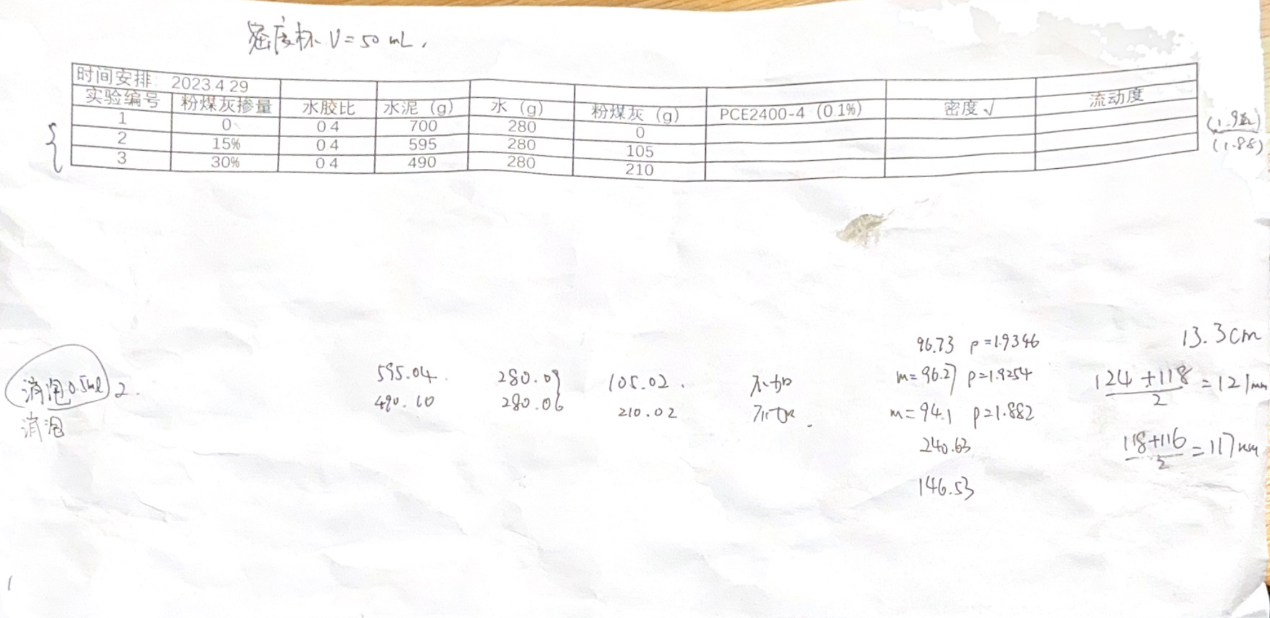
\includegraphics[width = 0.7 \linewidth]{figures/exp1/record table.png}
    \caption{实验数据记录表}
\end{figure}

\begin{figure}
    \centering
    \subcaptionbox{浆体流动性实验}{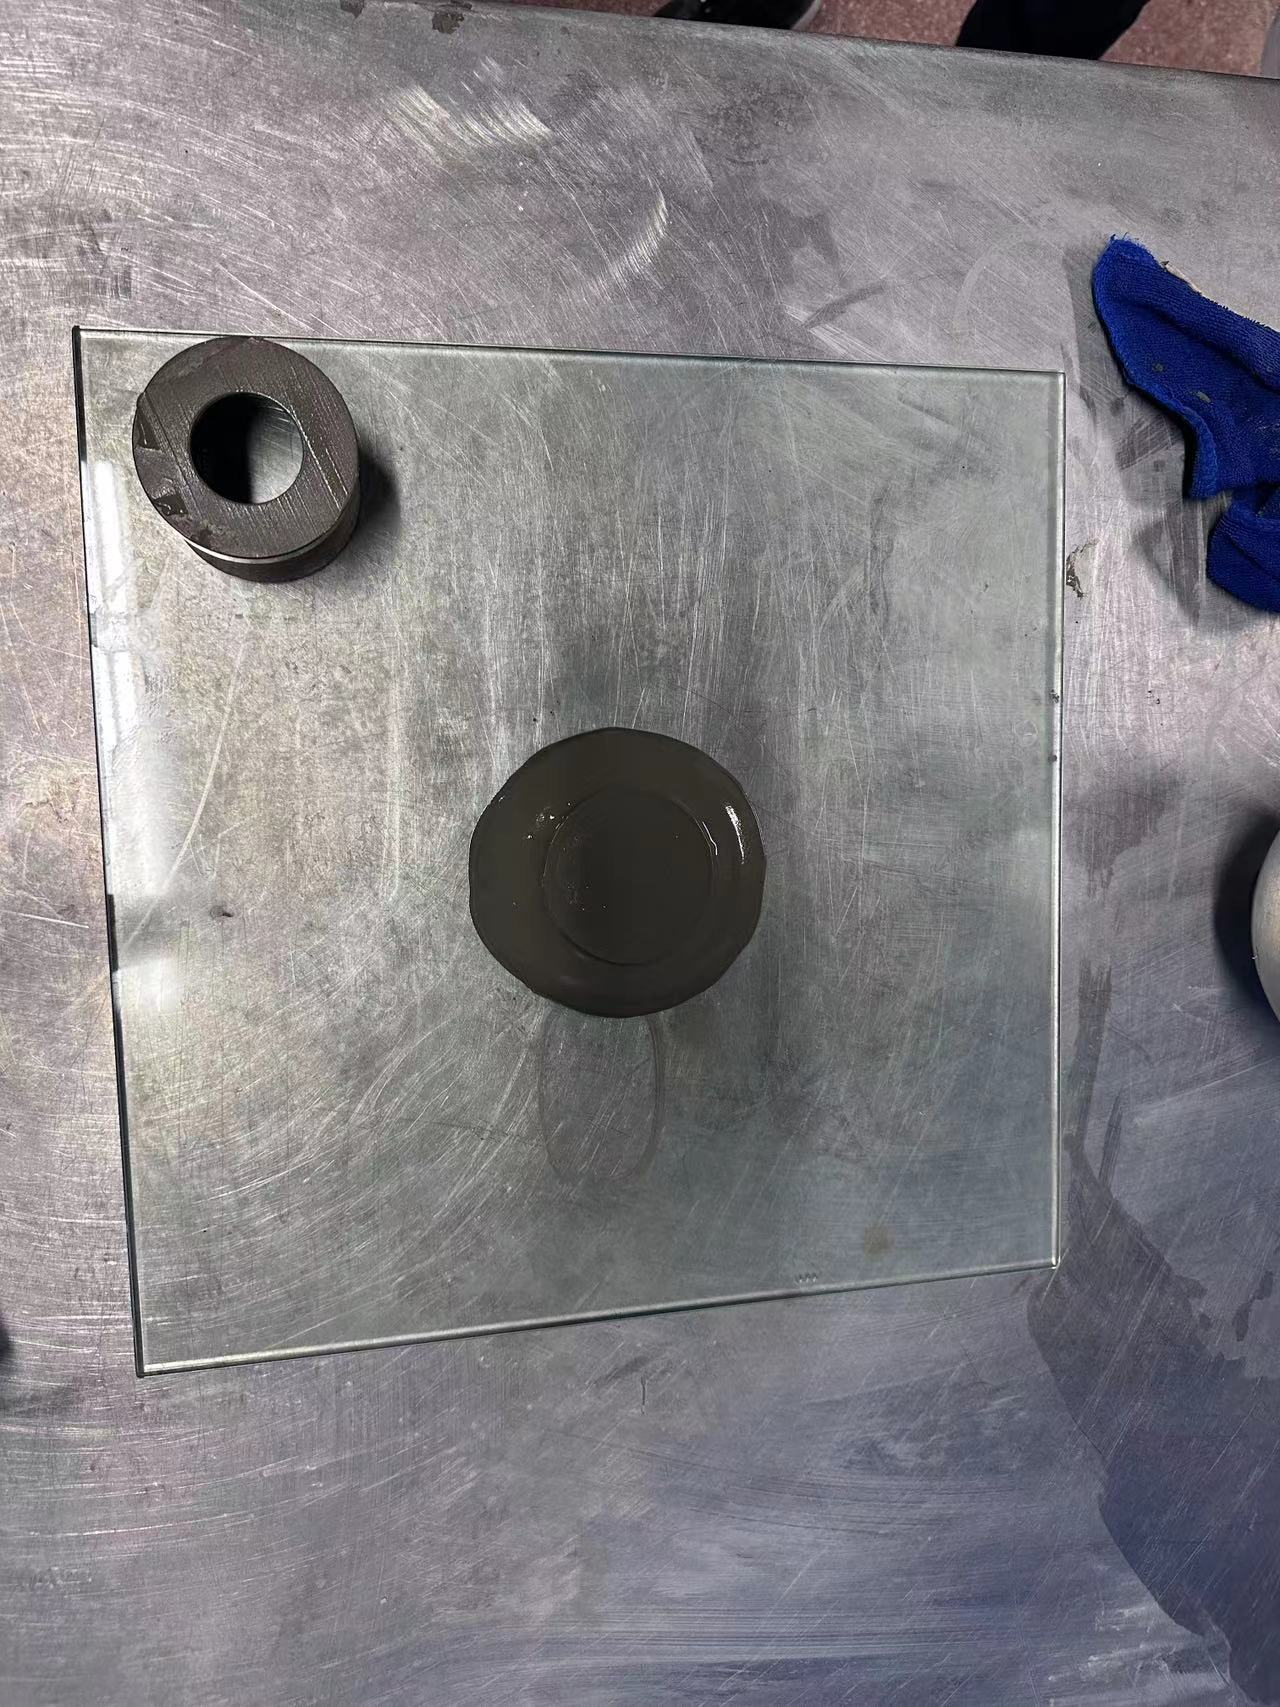
\includegraphics[height = 0.3 \linewidth]{figures/exp1/mobility.png}}\quad
    \subcaptionbox{测量浆体密度的不锈钢密度杯(图片来源于网络)}{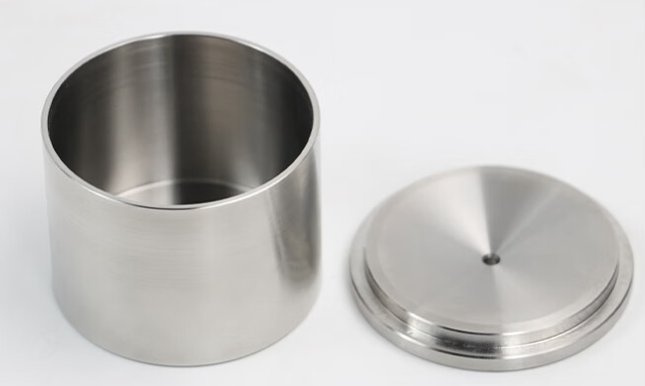
\includegraphics[height = 0.3 \linewidth]{figures/exp1/steel density cup.png}}
    \caption{浆体性质实验}
\end{figure}

\subsubsection{试块抗压强度试验}
试件成型 \SI{24}{\hour} 后拆模, 将其放入标准养护室中养护7d后测试其抗压强度.
使用试金\SI{300}{\kilo\newton}试验机进行水泥净浆试块抗压强度试验.该试验机最大荷载为 \SI{300}{\kilo\newton} , 最大位移为\SI{200}{\milli\meter} .
实验过程中应严格遵照试验机操作规程: 
\begin{enumerate}[wide, labelwidth=!, labelindent=0pt]
    \item 开动试验机之前, 先确保上下承压板之间无夹具和试样; 
    \item 启动计算机; 
    \item 启动计算机中的试验机测控软件; 
    \item 按下油源面板上的“电源开”、“油泵开”按钮; 
    \item 使用试验机测控软件的“砂浆抗压试验”控制模式, 将养护 \SI{7}{\day} 的各组 \qtyproduct{40 x 40 x 40}{\milli\meter} 水泥净浆试块置于试验机上, 进行试验; 
    \item 测试完成后, 按下油源面板上的“油泵关”、“电源关”按钮; 
    \item 关闭试验机的测控软件, 再关闭计算机! 
    \item 将测试用夹具从上下承压板之间取出; 
    \item 将废试样带走, 将试验机周边清理干净.
\end{enumerate}

设备使用过程中, 如出现任何非预期现象, 应立即按下油源面板上的“急停”按钮, 停止试验机运行! 

试验结果如表~\ref{tbl:compressive_strength_test}所示.

\han{(缺少了2-1的数据, 是不是当时少拍了?)}
\begin{table}[!t]
    \centering
    \caption{抗压强度测试结果}
    \begin{tabular}{|c|c|}
    \hline
    试样编号 & 抗压强度(\si{\mega\pascal}) \\ \hline
    1-1  & 39.2      \\ \hline
    1-2  & 36.5      \\ \hline
    3-1  & 30.6      \\ \hline
    3-2  & 30.7      \\ \hline
    \end{tabular}
    \label{tbl:compressive_strength_test}
\end{table}

\subsection{通过 SEM 观察水泥净浆试块断面的微观形貌}

将水泥净浆试块在标准养护室养护至 \SI{7}{\day} 之后, 一部分直接取断面观察其微观形貌.
方法如下: 取试块中央部分剪成黄豆粒大小的薄片, 并在异丙醇中浸泡 \SI{24}{\hour} 以终止水化; 对随后取出置于 \SI{40}{\degreeCelsius} 的真空烘箱中烘干 \SI{24}{\hour}, 之后对样品进行喷金处理, 最后置于 SEM 下观察其微观形貌. 

本实验使用场发射环境扫描电子显微镜. 等压强的数值下降到 \num{3e-3} 点亮HV (High Voltage), 然后再在显微镜下找到样品位置, 接着选择合适的放大倍数, 最后对焦并保存图片. 
如果需要了解指定区域的元素组成, 需要在影像中选取研究区域, 得到其对应能谱图.

\begin{figure}
    \centering
    \subcaptionbox{能谱图}{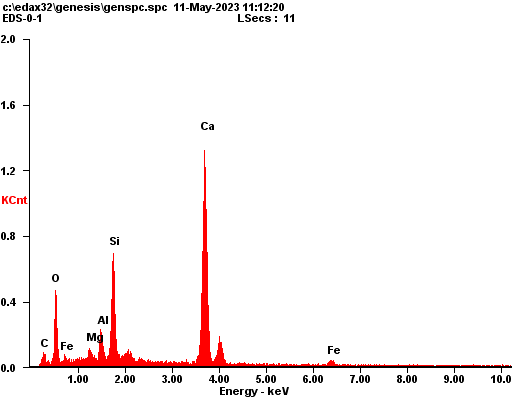
\includegraphics[height = 0.3 \linewidth]{assets/spectrum/00-01-10000x-ETD-C3S.png}} \quad
    \subcaptionbox{ETD图像及选择区域}{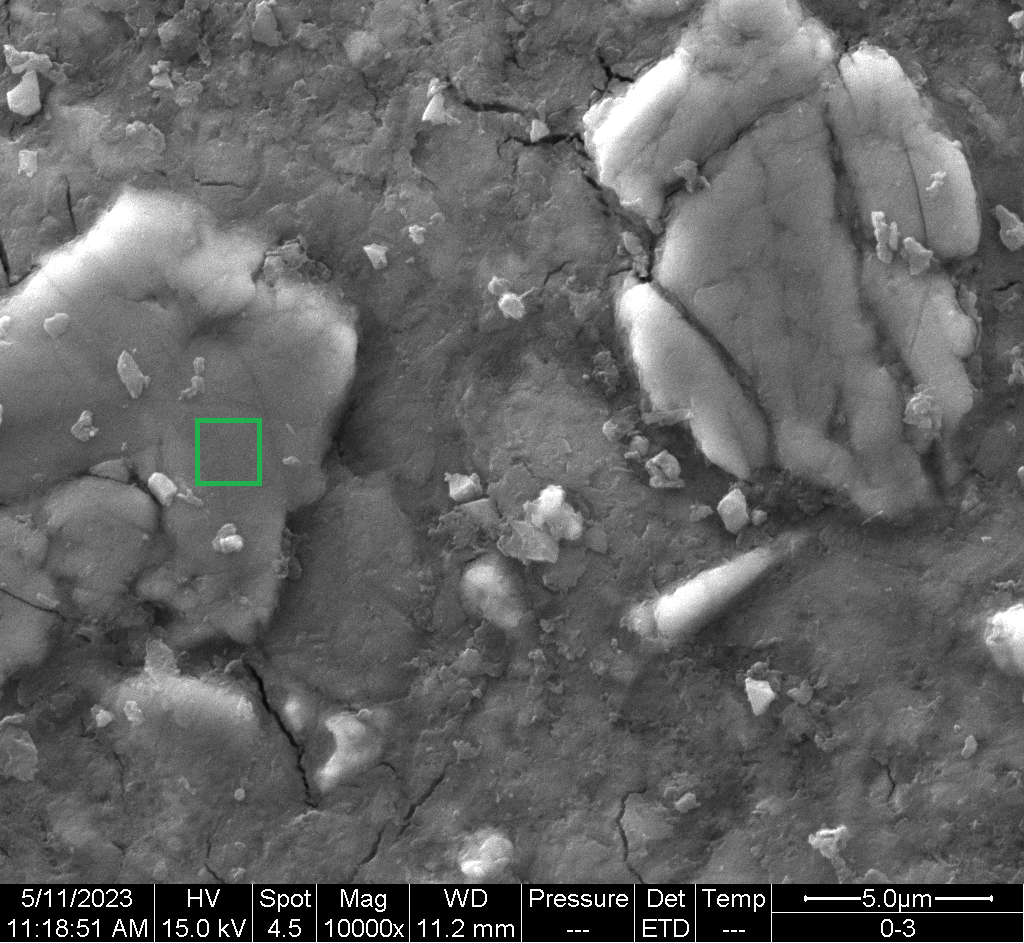
\includegraphics[height = 0.3 \linewidth]{assets/spectrum selection/00-01-10000x-ETD-C3S.png}}
    \caption{样品图像及其能谱图. 考虑钙、硅的物质的量之比, 该区域成分应该是 \ce{C3S} .}
\end{figure}

\subsection{观察抛光样品的背散射电子成像}

将水泥净浆试块在标准养护室养护至 \SI{7}{\day} 之后, 取另一部分水泥净浆样品浸泡在异丙醇中以终止水化, 然后在 \SI{40}{\degreeCelsius} 的真空烘箱中烘干 \SI{24}{\hour}, 之后取出将其嵌入环氧树脂中进行抛光处理. 具体而言, 利用 \SI{400}{\text{目}} 的砂纸进行粗抛光, 持续 \qtyrange{1}{2}{\minute} , 再利用 \SI{5000}{\text{目}} 的砂纸进行细抛, 持续时间 \SI{5}{\minute} , 最后利用附着 \SI{1}{\micro\meter} 金刚石喷雾的抛光绒布进行精抛. 
之后对样品进行喷金处理, 使用环氧树脂(AB胶)和硅胶模具进行金相制样, 等待环氧树脂完全硬化. 
最后置于 SEM 下观察其背散射电子成像.


\begin{figure}[!t]
    \centering
    \subcaptionbox{抛光用的砂纸}{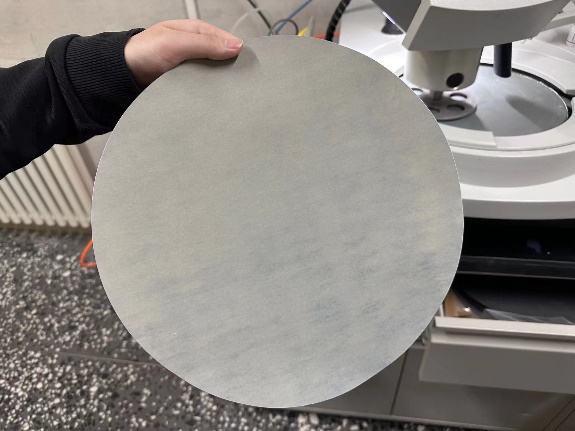
\includegraphics[height = 0.3 \linewidth]{figures/exp3/sandpaper.png}} \quad
    \subcaptionbox{抛光用的绒布}{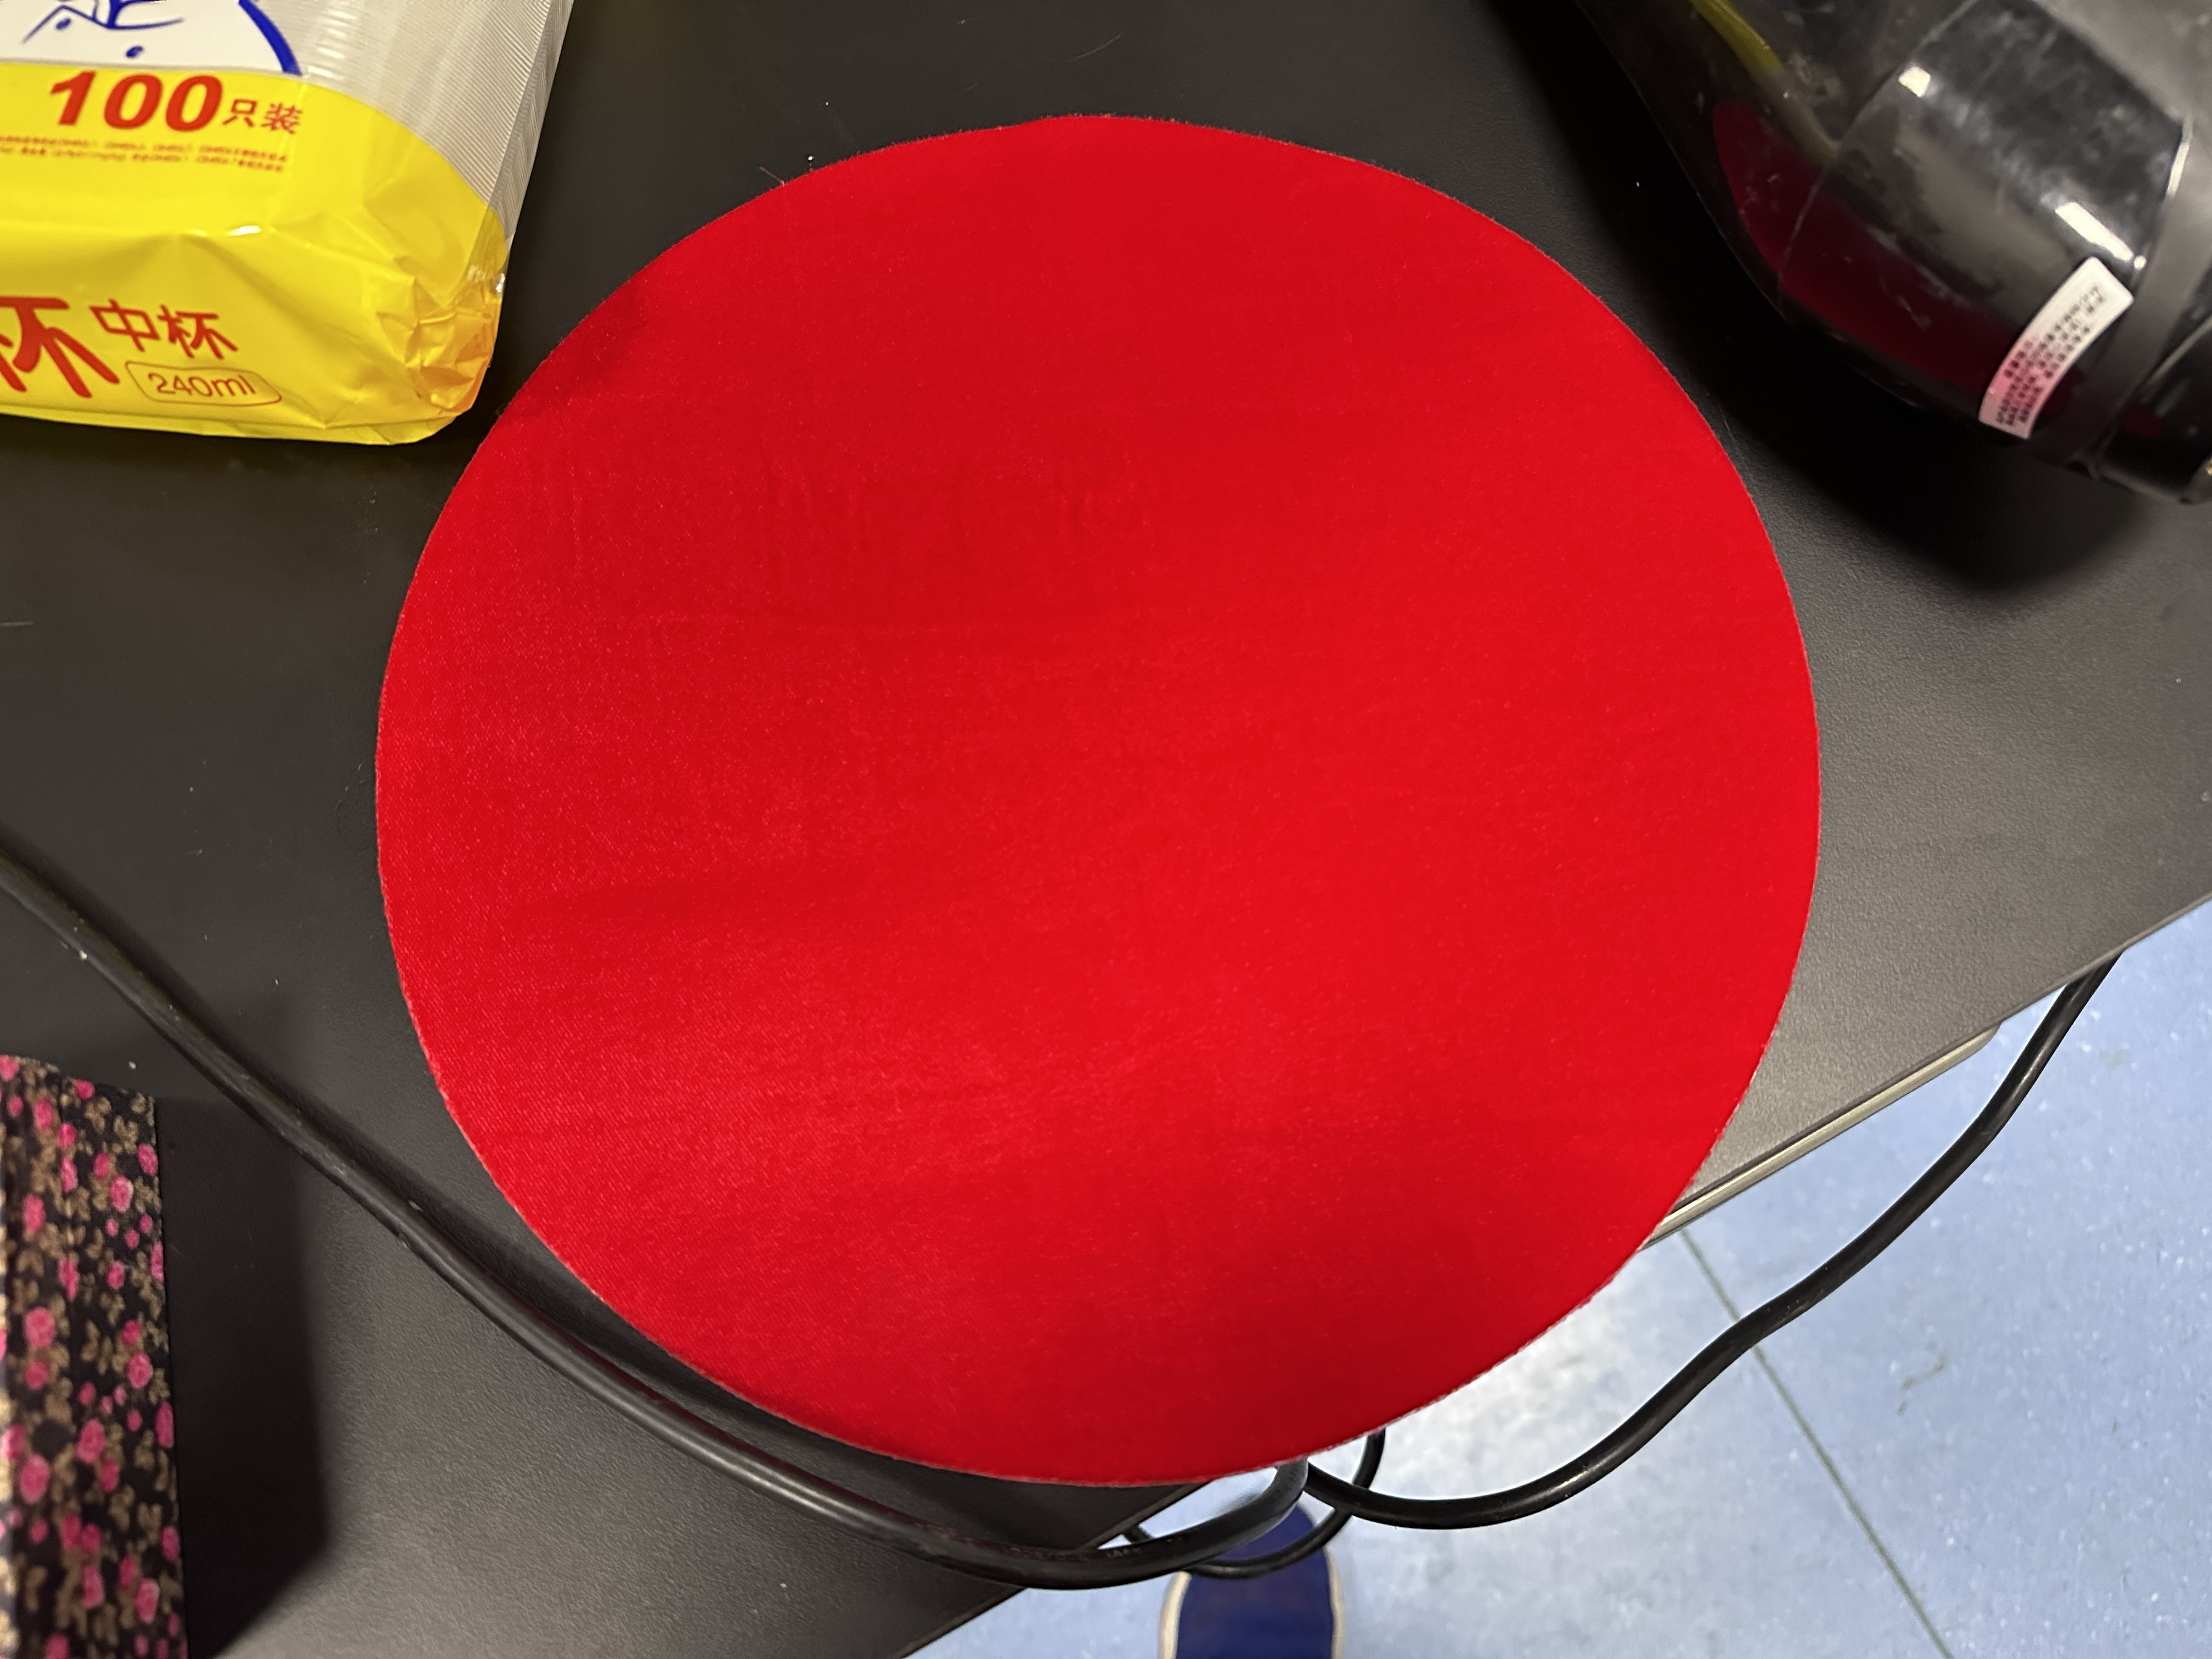
\includegraphics[height = 0.3 \linewidth]{figures/exp3/flannel.png}} \quad
    \subcaptionbox{抛光剂}{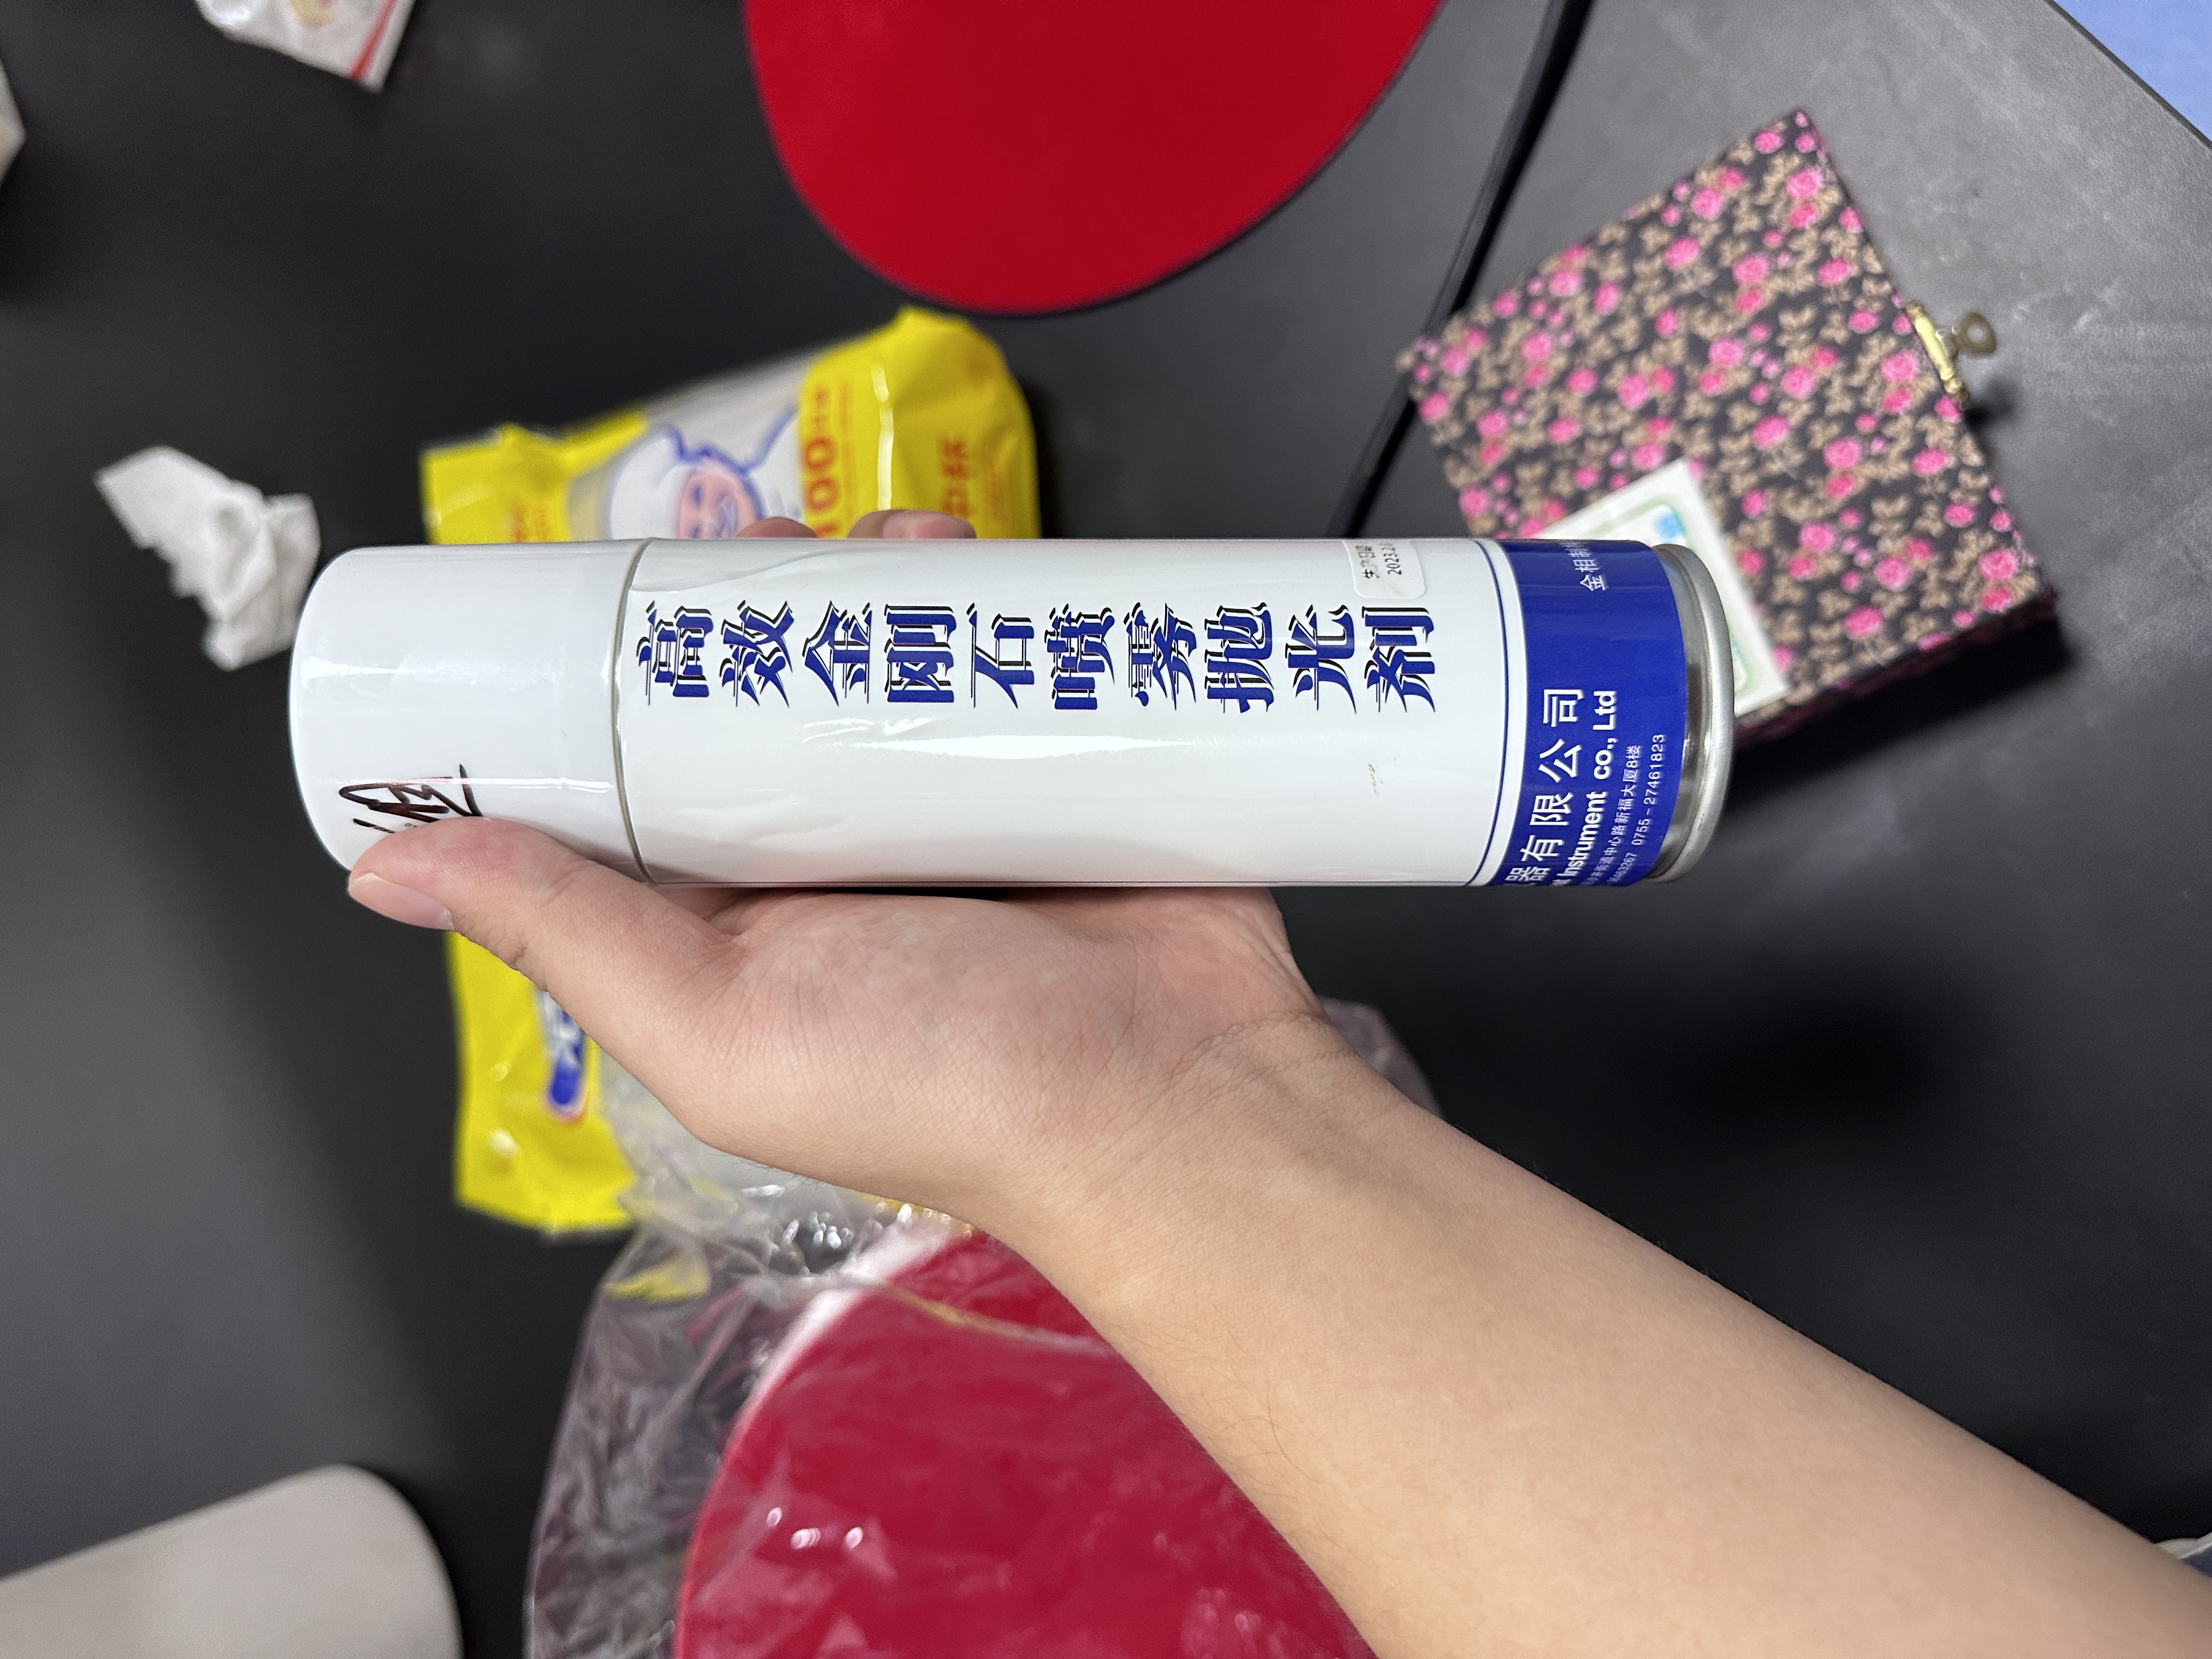
\includegraphics[height = 0.3 \linewidth]{figures/exp3/polish.png}}
    \caption{样品抛光用的器具}
\end{figure}

\begin{figure}[!t]
    \centering
    \subcaptionbox{抛光机}{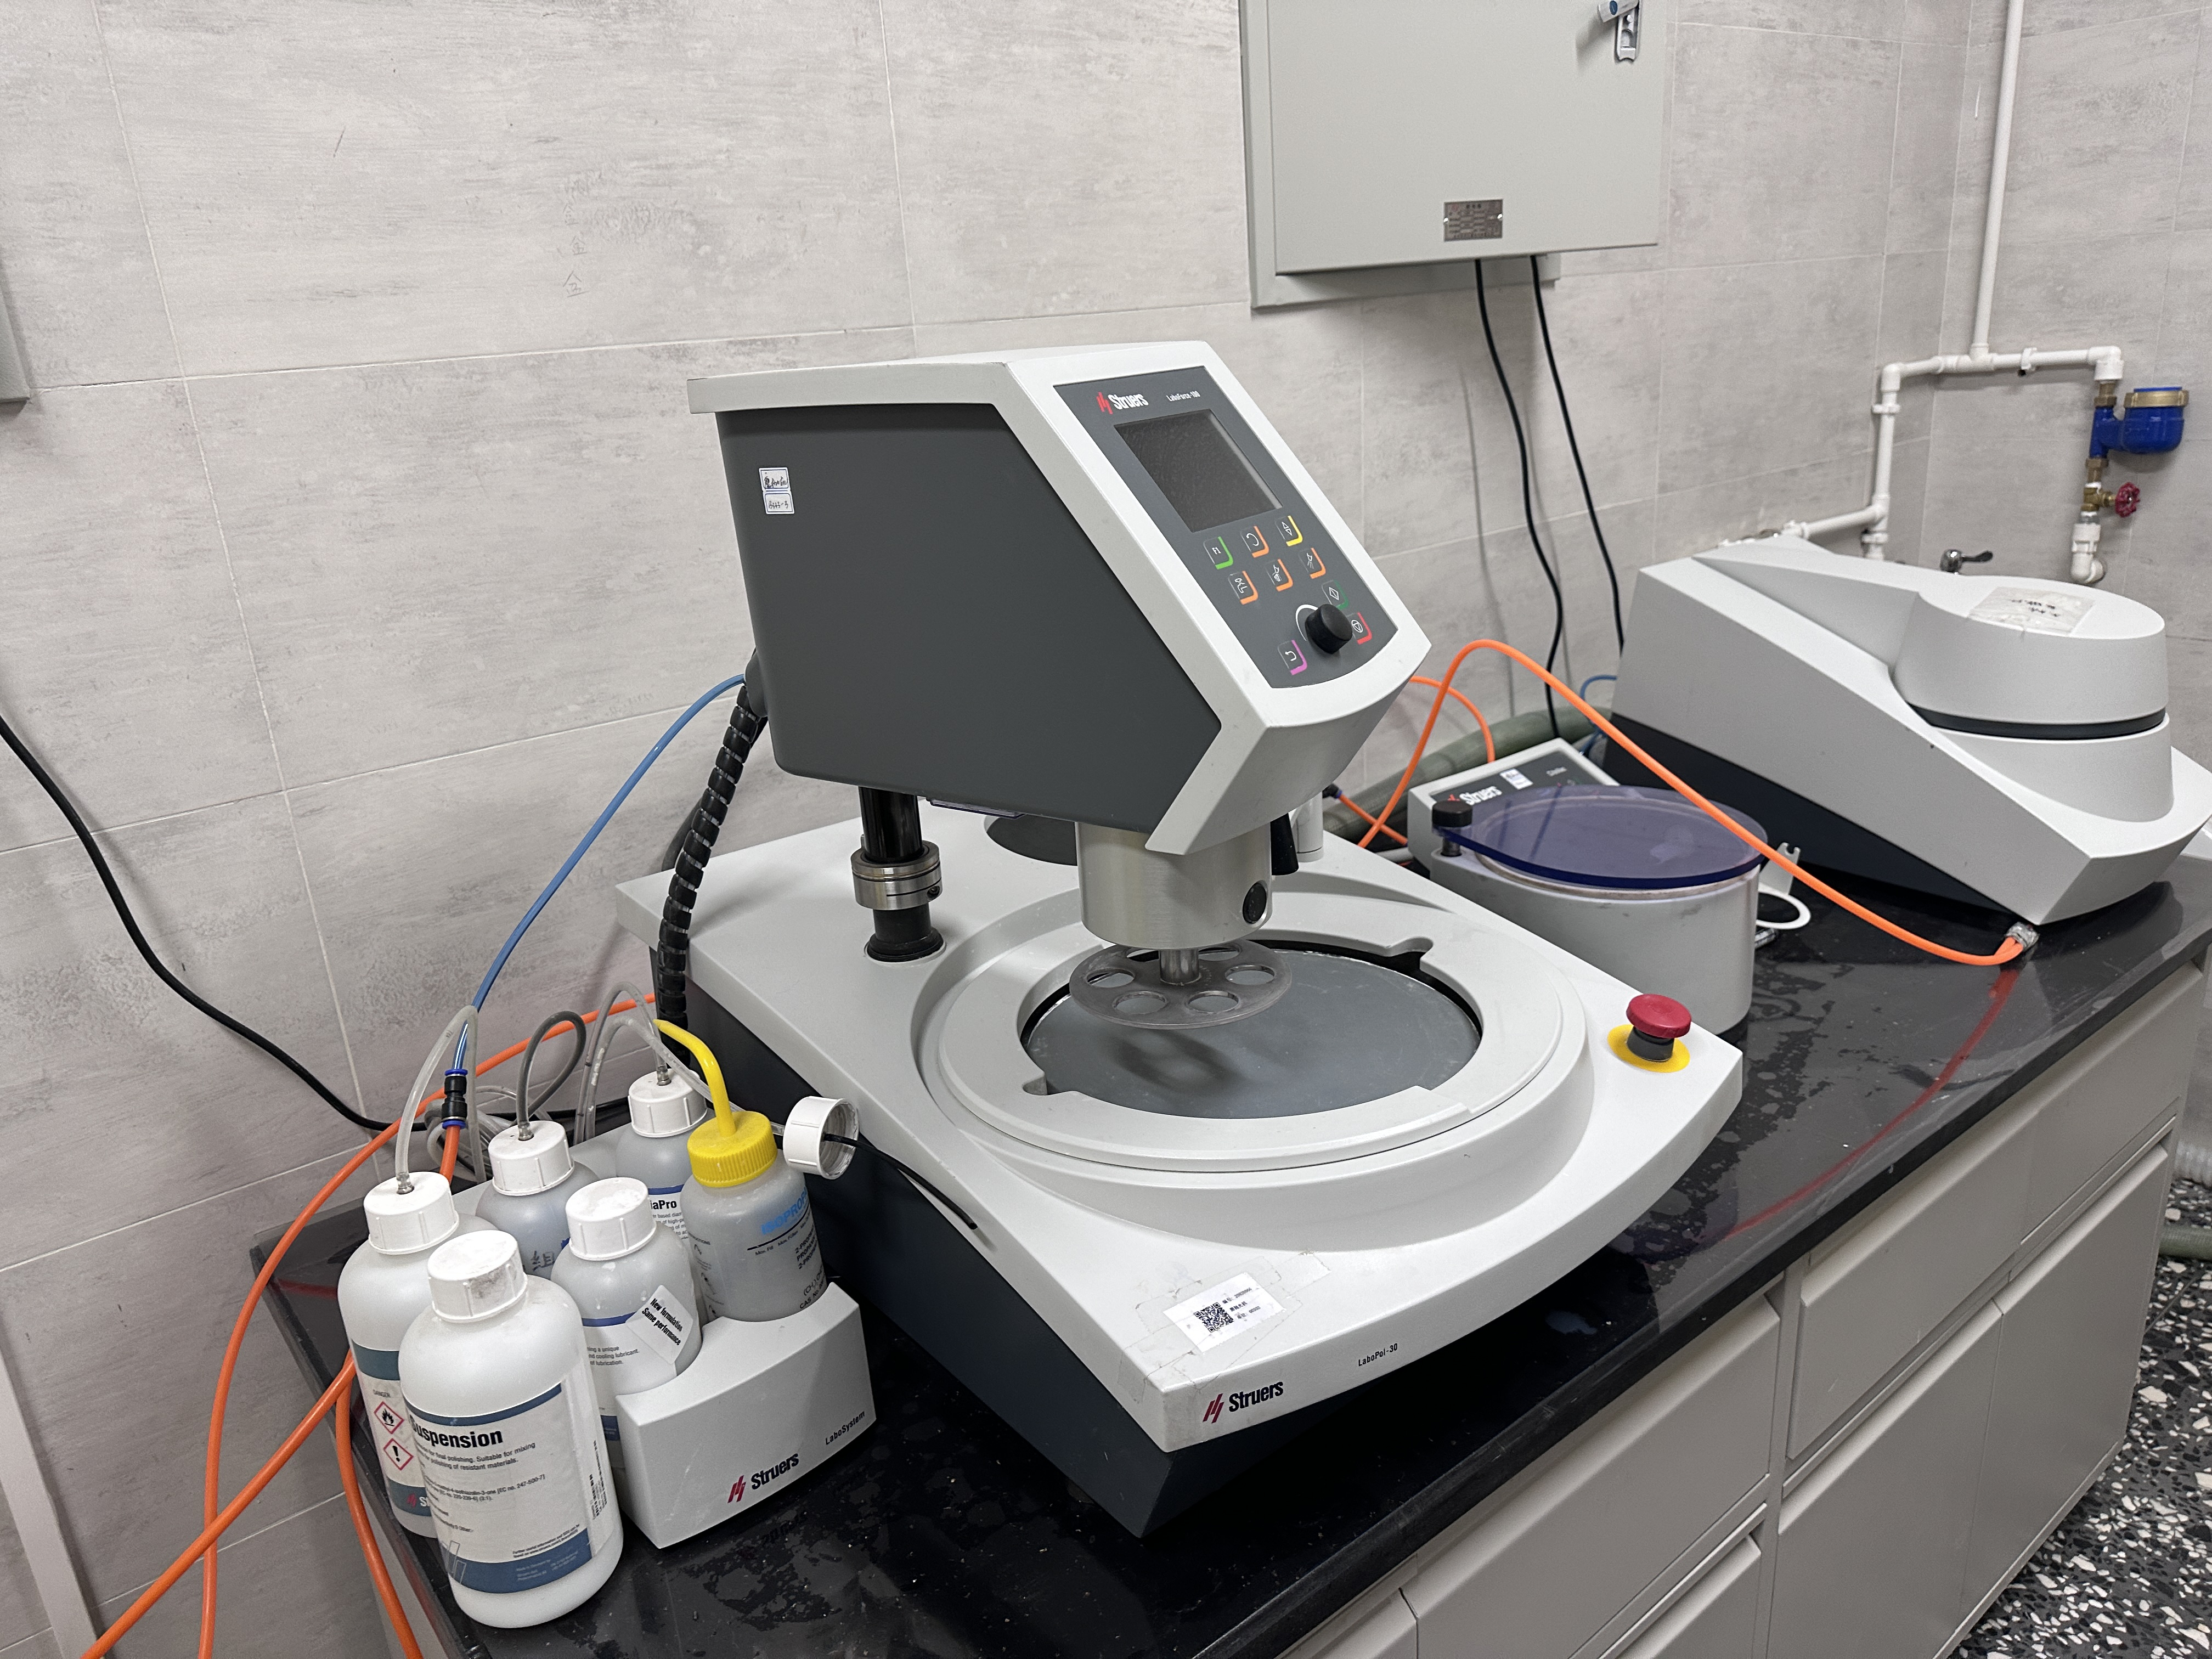
\includegraphics[height = 0.3 \linewidth]{figures/exp3/polish machine.png}} \quad
    \subcaptionbox{抛光成品}{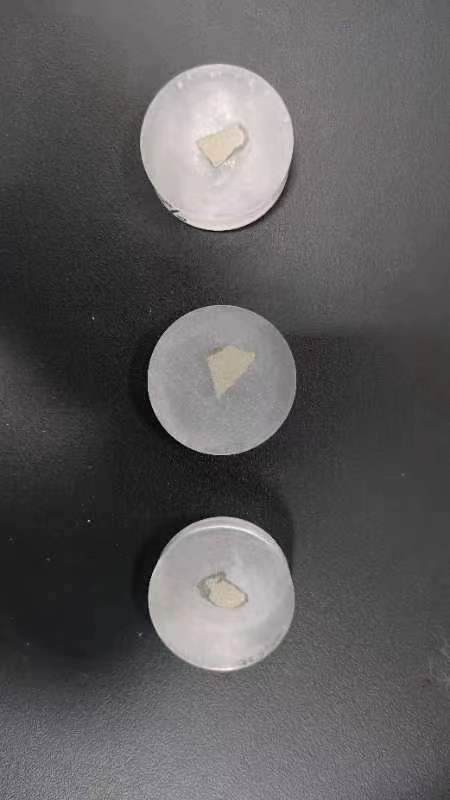
\includegraphics[height = 0.3 \linewidth]{figures/exp3/polished sample.png}}
    \caption{抛光用的仪器和成品}
\end{figure}


\begin{figure}
    \centering
    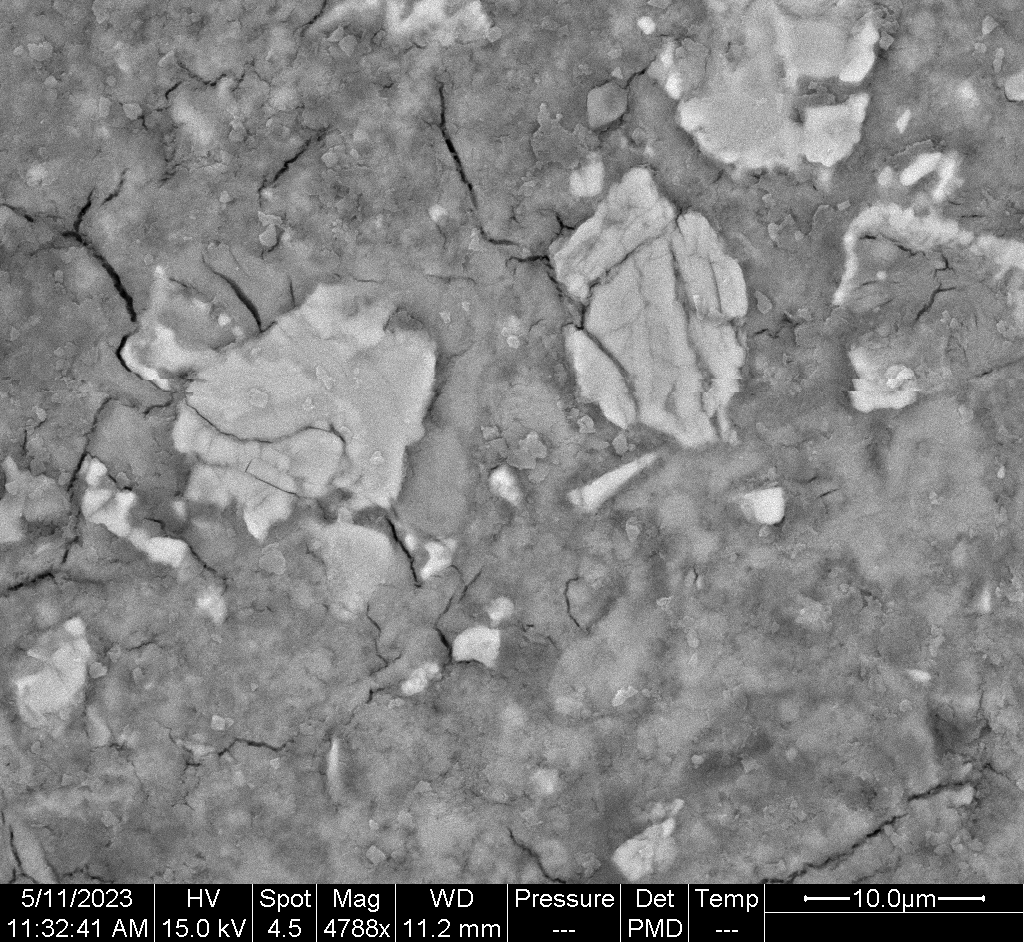
\includegraphics[width = 0.4 \linewidth]{assets/00-polished-04788x-PMD.png}
    \caption{粉煤灰掺量为 \SI{0}{\percent} , 抛光后的硬化水泥块, 在 4788x 放大下的背散射图.在背散射图中, 原子序数越高, 亮度越高. 由于水泥中原子序数最高的是钙元素, 所以含钙量高的地方最亮. }
\end{figure}


\han{(我把剩下的图片和当时简单记录的结果也都放在下面了, 分析实验结果的时候可以参考)}